\documentclass[11pt]{report}
\usepackage{graphics}
\usepackage{graphicx}
\usepackage{epsfig}
\usepackage{fancyhdr}
%\usepackage{fullpage}
\usepackage{float}
\usepackage{xspace}
%\usepackage{algorithm}
%\usepackage{algorithmic}
%\usepackage{algorithmicx}

\begin{document}
\renewcommand\bibname{References}
\pagestyle{fancy}
%\fancyheadz{}
\fancyfoot{}
\fancyfoot[c]{\thepage}
\fancyfoot[l]{CSD334-Mini Project 2022}
\lhead{abcd}
\renewcommand{\chaptermark}[1]{
\markboth{\thechapter.\ #1}{}} 
\renewcommand{\headrulewidth}{0.1pt}
\fancyhead[r]{\slshape \leftmark}
\addtolength{\headheight}{\baselineskip}

\lhead{\nouppercase{\rightmark}}
\rhead{\nouppercase{\leftmark}}
%\lhead{hhhhh}
%\fancyhead[LO,RE]{\slshape \leftmark}
%\bibliographystyle{plain}
\title {E-Kart}
\author {Jaison Dennis}
%\maketitle

\begin{titlepage}
\begin{center}

%\topmargin100pt
\Huge{\textbf{E-MART}}\\
\large{\textbf{\\CSD334-Mini Project 2022\\}}
\vspace{1.2in}
\Large{\textbf{Jaison Dennis}}\\ 
\Large{\textbf{20CSA34\\
MDL20CS060\\
}}	\hspace{.1in}	

\Large{\textbf{
\\B. Tech. Computer Science \& Engineering
}}


\vspace{.6in}
\begin{figure}[h]
\begin{center}
%\epsfig{width=1in, file=embN1.jpg}

\epsfig{width=1in, file=logo.jpg}
% If you have access to better quality logo image, that may be used, but all the groups should use the same image
\end{center}
\end{figure}
%\vspace{.2in}
\textbf{
Department of Computer Engineering\\
Govt. Model Engineering College Thrikkakara\\
Thrikkakara, Kochi 682021\\
Phone: +91.484.2575370\\
http://www.mec.ac.in \\
hodcs@mec.ac.in
}
\end{center}
\end{titlepage}




\begin{titlepage}
\begin{center}
\Large{\textbf{Govt. Model Engineering College Thrikkakara}}\\
\Large{\textbf{\\Dept. of Computer Engineering}}\\
\end{center}
\begin{figure}[h]
\begin{center}

\epsfig{width=1in, file=logo.jpg}
\end{center}
\end{figure}
\begin{center}
\Large{\textbf{C E R T I F I C A T E}}\\
\vspace{.1in}
\end{center}
This is to certify that, this report titled \textbf{\textit {E-MART}} is a bonafide record of the work done by
{\textbf{20CSA34
MDL20CS060
}{\textbf{Jaison Dennis}}} {{, \textbf{Fifth Semester} B. Tech. Computer Science \& Engineering }}
student,  for the course work in \textbf{CSD334-Mini Project 2022} which is the Mini Project Work, under our guidance and supervision, in partial 
 fulfillment of the requirements for the award of the degree, B. Tech. Computer 
Science  and Engineering of \textbf{APJ Abdul Kalam University }.
\vspace{.1in}
\begin{tabbing}
xxxxxxxxxxxxxxxxxxxxxxxxxxxxxxxxxxxxxxxxxxxxxxx\= xxxxxxxxxxxxxxxxxx\= \kill

						Coordinator	\>Head of the Department
\\
\\
\\
  Veena Briji Philip\>Dr.Preetha Theresa Joy\\
	Assistant Professor\>Head of the Department
	
	 \\
	 \>Professor\\
Computer Engineering	\>	Computer Engineering
\end{tabbing}
\vspace{.08in}
%
\begin{tabbing}
xxxxxxxxxxxxxxxxxxxxxxxxxxxx\= xxxxxxxxxxxxxxxxxx\= \kill
			 \\
\\
\\
\today
\end{tabbing}
\end{titlepage}

\begin{center}
	\thispagestyle{empty}
	\LARGE{\textbf{Acknowledgements}}\\[1cm]
\end{center}
\linespread{1.13}
\large{\paragraph{}We would like to express deepest appreciation towards \textbf{Dr.Jacob Thomas},
	Principal, Govt. Model Enginnering College , Thrikkakara, \textbf{Prof. Preetha Theresa Joy}, 
	Head of Department of Computer Engineering and \textbf{Mrs.Veena Briji Philip }, Project Coordinator whose
	invaluable guidance supported us in completing this project.}
\large{\paragraph{}At last we must express our sincere heartfelt gratitude to all the staff members
	of Computer Engineering Department who helped me directly or indirectly during this course of work.}
\begin{flushright}
	{
		Jaison Dennis\\
		Jagannath E Shahi\\
		Christopher Roy
	}
\end{flushright}
\newpage
 
\begin{abstract}
\pagenumbering{roman}
This project 'E-Mart' is an e-commerce platform  which sells its goods and services online making it easier for the user to access a wide variety of items from a single platform. E-Mart allows customers to browse and purchase products from a variety of sellers through a web browser. The platform handles all aspects of the transaction, including payment processing, order fulfillment, and order tracking. The platform may also offer features such as personalized recommendations, wish lists, and reviews to help customers find the products they are looking for. Users can also add products to cart and buy them at a later time. Users can search and filter products based on price, brand and offers. Our platform is open for both end users and sellers. The goal of the platform is to create a convenient and easy-to-use shopping experience for customers, while also providing a means for sellers to reach a larger audience and grow their businesses.
\end{abstract}

\tableofcontents





\chapter {Introduction}
\pagenumbering{arabic}
\label{intro}
An online e-commerce platform is a digital marketplace that enables businesses and individuals to sell products and services to customers over the internet. The platform provides a central location for sellers to list their products, and for customers to browse and make purchases. With the increasing popularity of online shopping, the demand for convenient and reliable e-commerce platforms has grown significantly. Online shopping allows you to shop anytime, anywhere, as long as you have an internet connection. This is especially convenient for people with busy schedules or those who live in rural areas with limited access to physical stores.\\
\\It also have a much wider selection of products than traditional brick-and-mortar stores. This is because they do not have the same space constraints and can offer a larger inventory. In addition, online retailers often offer products from a variety of brands and manufacturers, giving you more options to choose from. Online retailers often have lower overhead costs, such as rent and utilities, which allows them to offer competitive prices. In addition, it is easy to compare prices from different online retailers to find the best deal. Online e-commerce platforms allow customers to leave reviews of products, which can be helpful in making informed purchasing decisions and provide valuable insights into the quality and functionality of a product, as well as any potential issues. Online retailers often have more lenient return policies, making it easier to return or exchange items that are not satisfactory.  Online e-commerce platforms can use your purchase history and browsing data to make personalized product recommendations, which can save you time and help you discover required products.


\section{Proposed Project}
\subsection{\label{ps}Problem Statement}

\subsection{Proposed Solution}
This should clearly, without any scope for differing interpretations later, state the methods you are suggesting to achieve the result.
\chapter{\label{work}Report of Preparatory Work }
%\section{\label{work}Report of Work Done}
\subsection{System Study Report}

%...............................................................................................


\chapter{Project Design}
 \label{xx}

\section{High Level Design}
\section{Block Diagrams}


\section{Algorithms}

\section{Hardware \& Software Requirements}
\section{Work Schedule}

\chapter{Screenshots}
\begin{figure}[H]
	\fbox{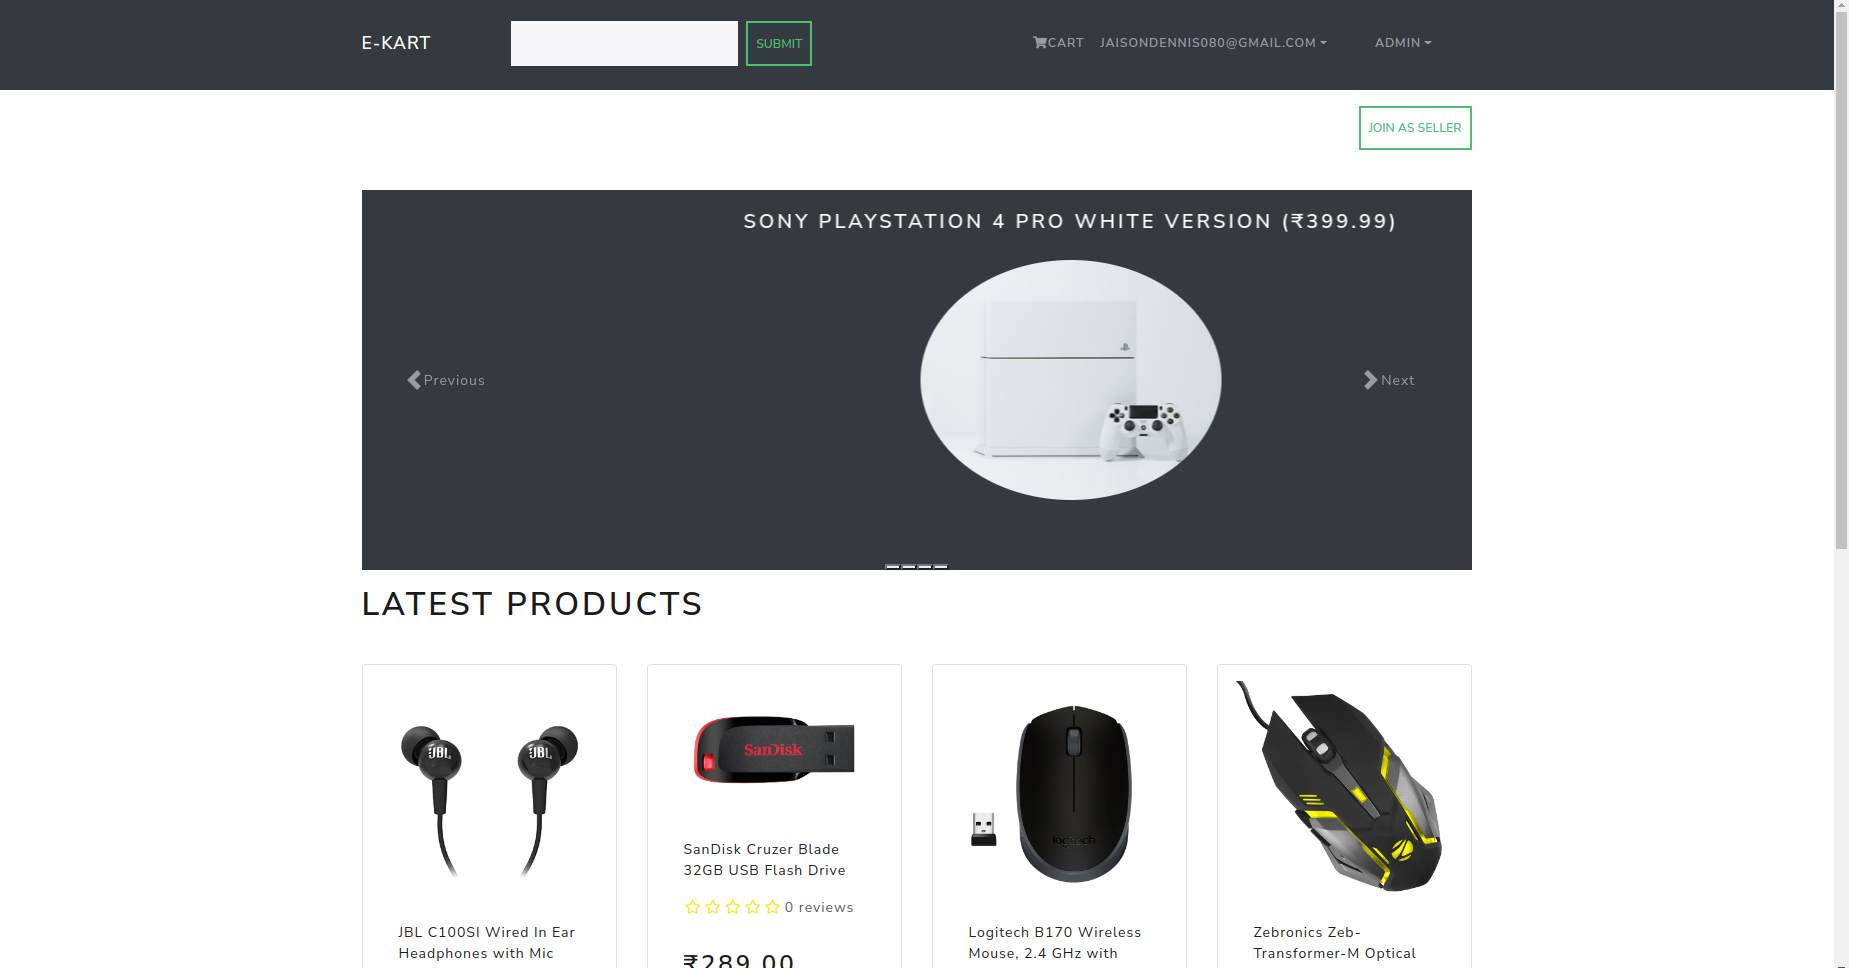
\includegraphics[width=\linewidth]{home.png}}
	\caption{Home Screen}
	\label{fig:erd}
\end{figure} 
\begin{figure}[H]
	\fbox{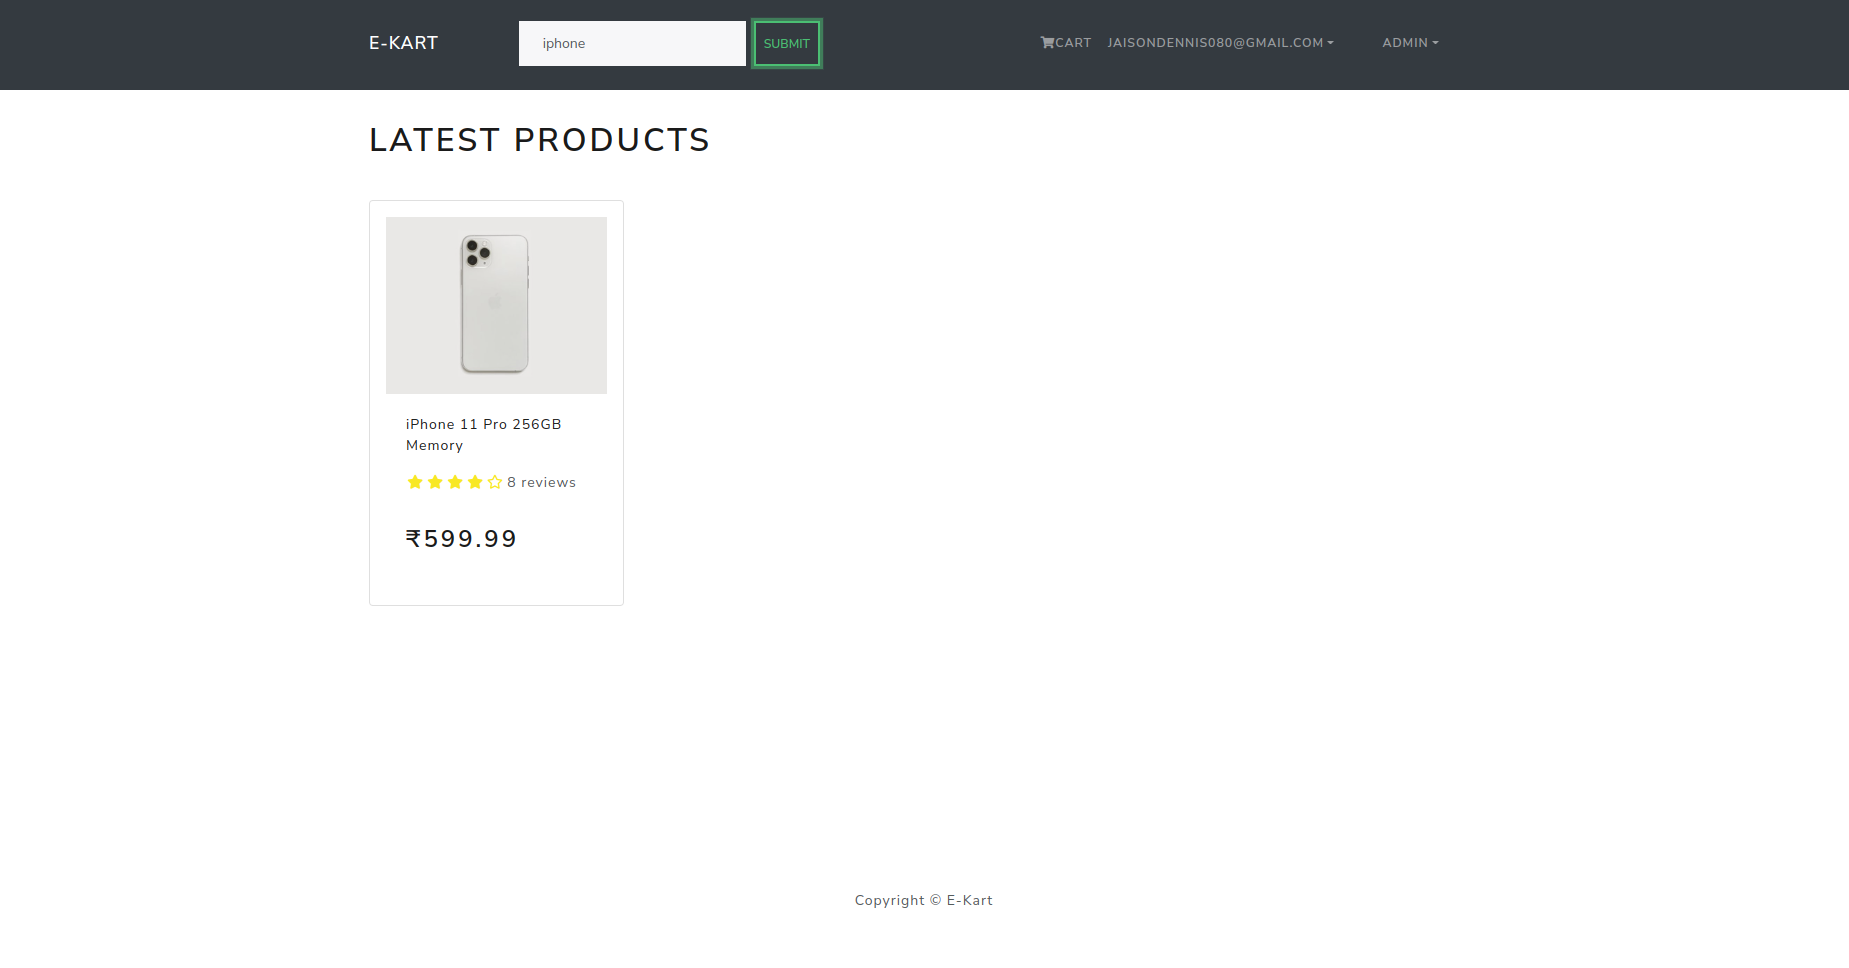
\includegraphics[width=\linewidth]{search.png}}
	\caption{Search Products}
	\label{fig:dfd}
\end{figure}
\begin{figure}[H]
	\fbox{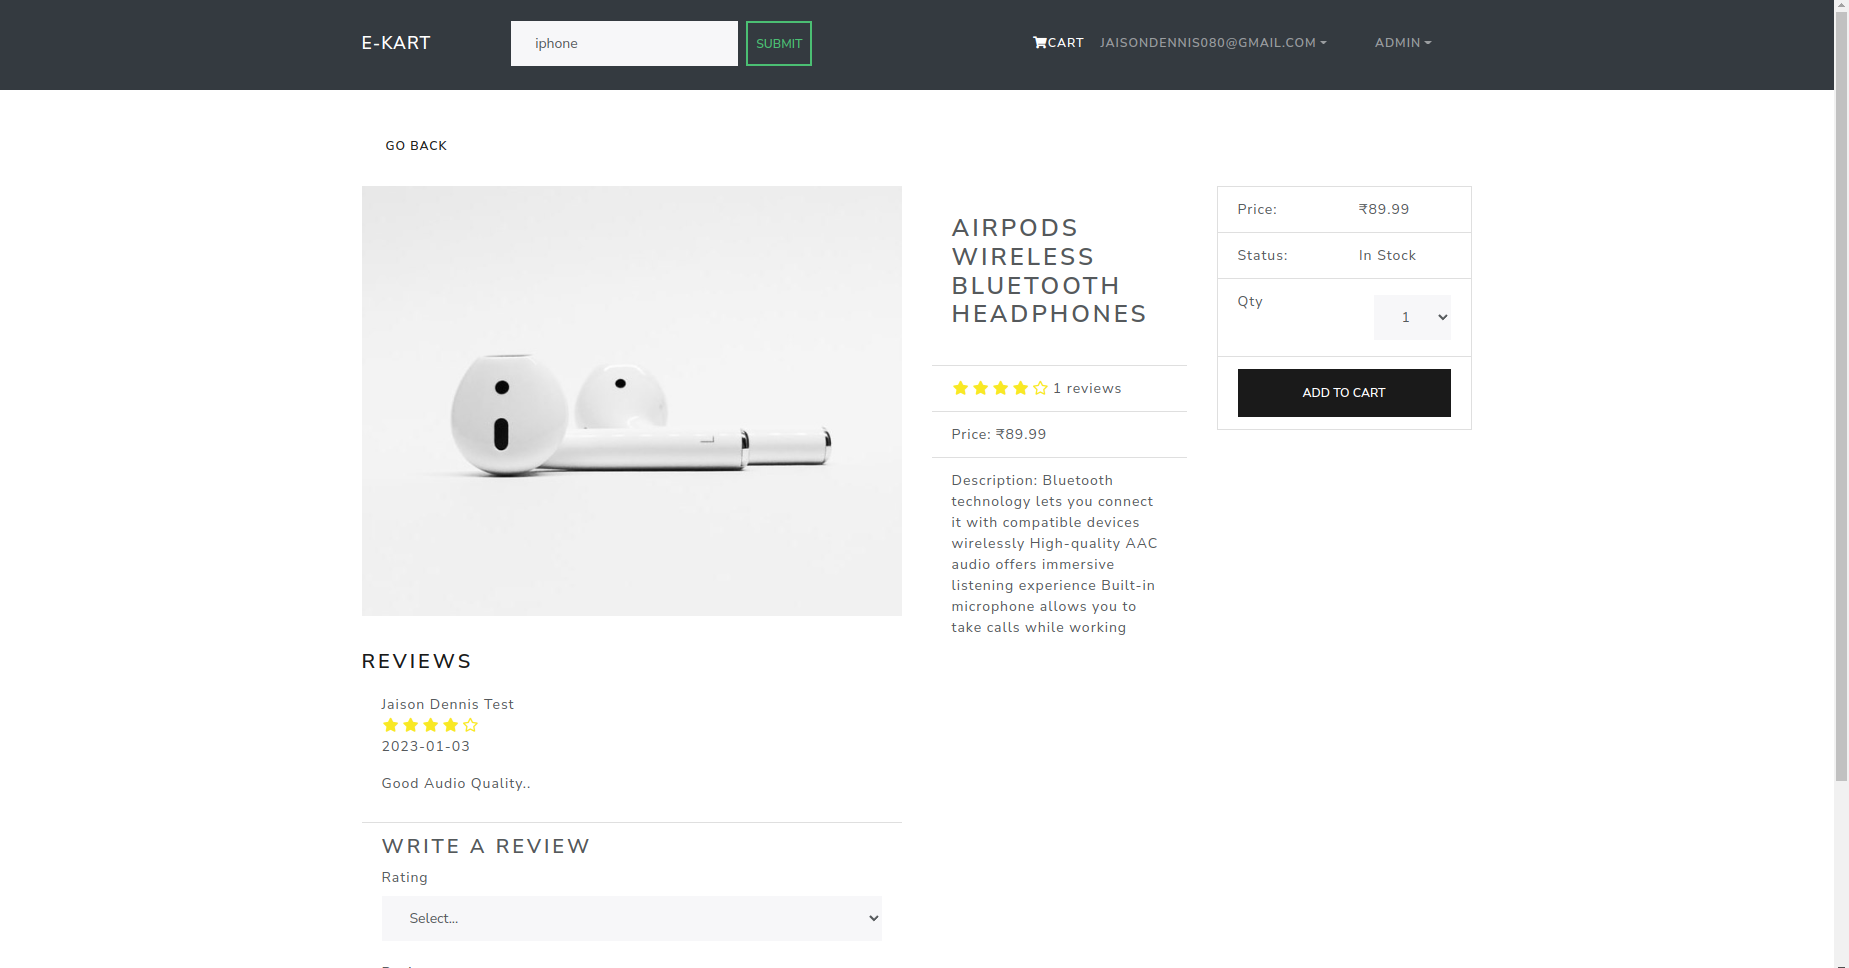
\includegraphics[width=\linewidth]{description.png}}
	\caption{Product Description}
	\label{fig:dfd2}
\end{figure}
\begin{figure}[H]
	\fbox{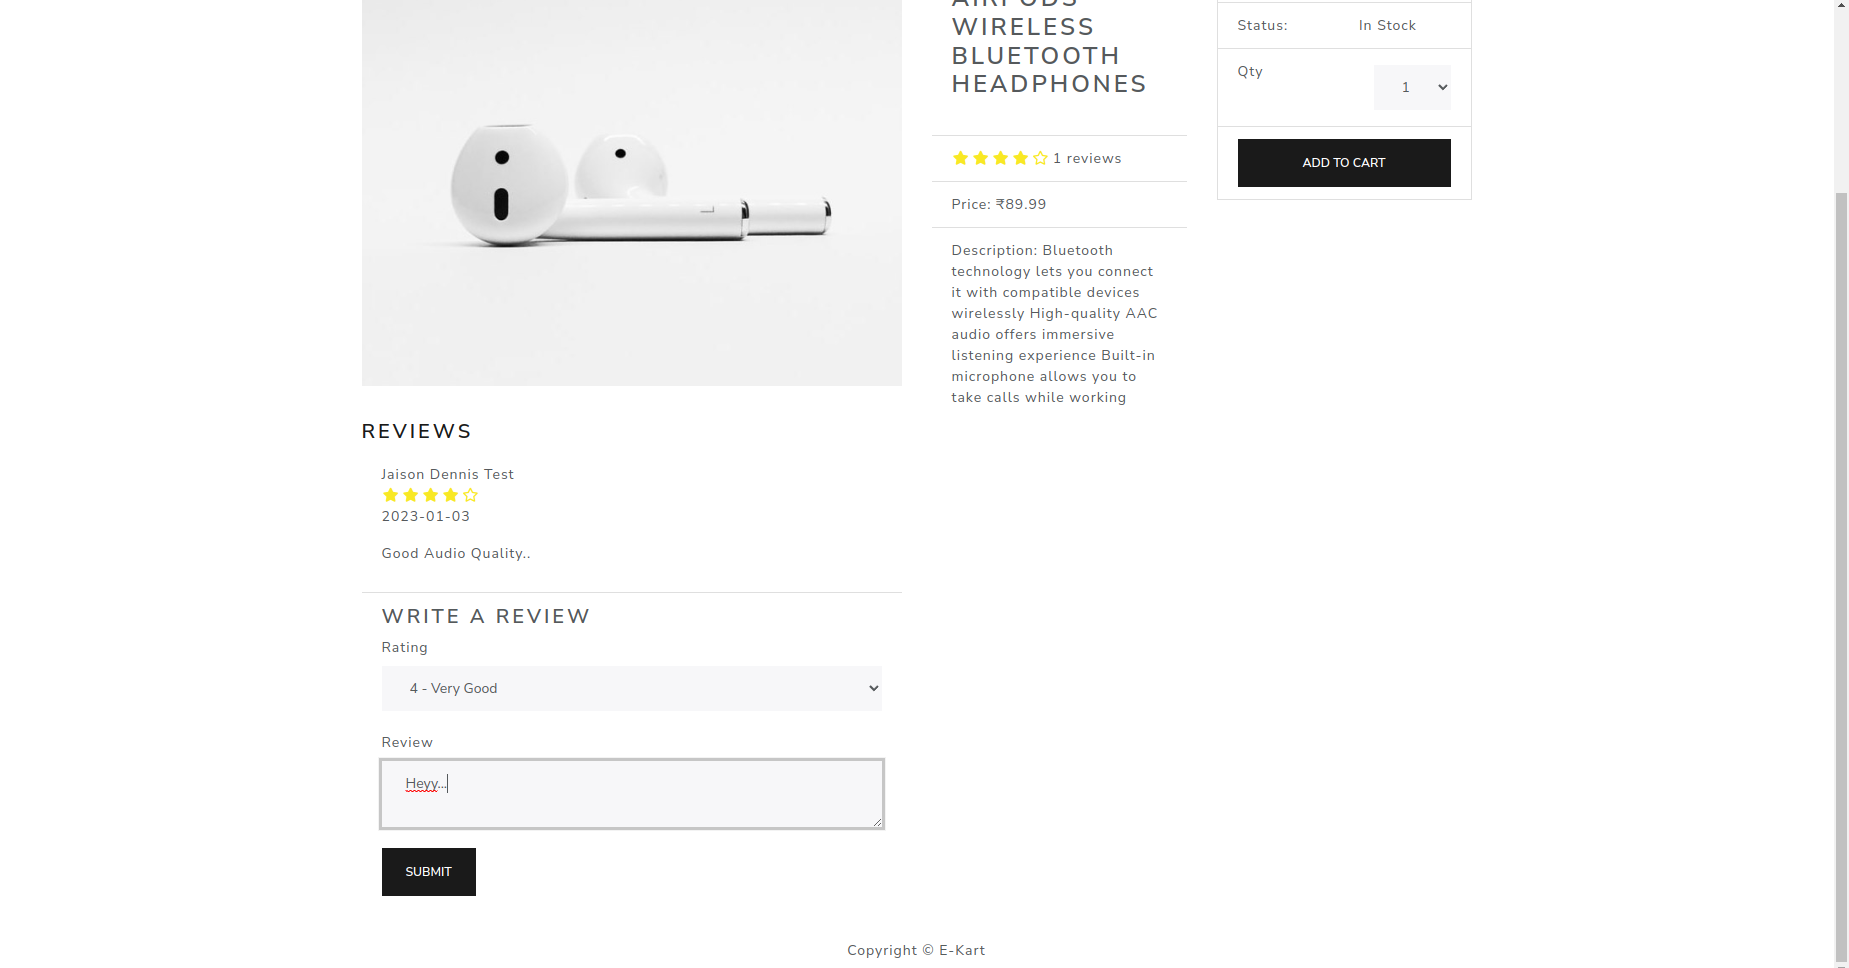
\includegraphics[width=\linewidth]{review.png}}
	\caption{Reviews}
	\label{fig:dfd3}
\end{figure}
\begin{figure}[H]
	\fbox{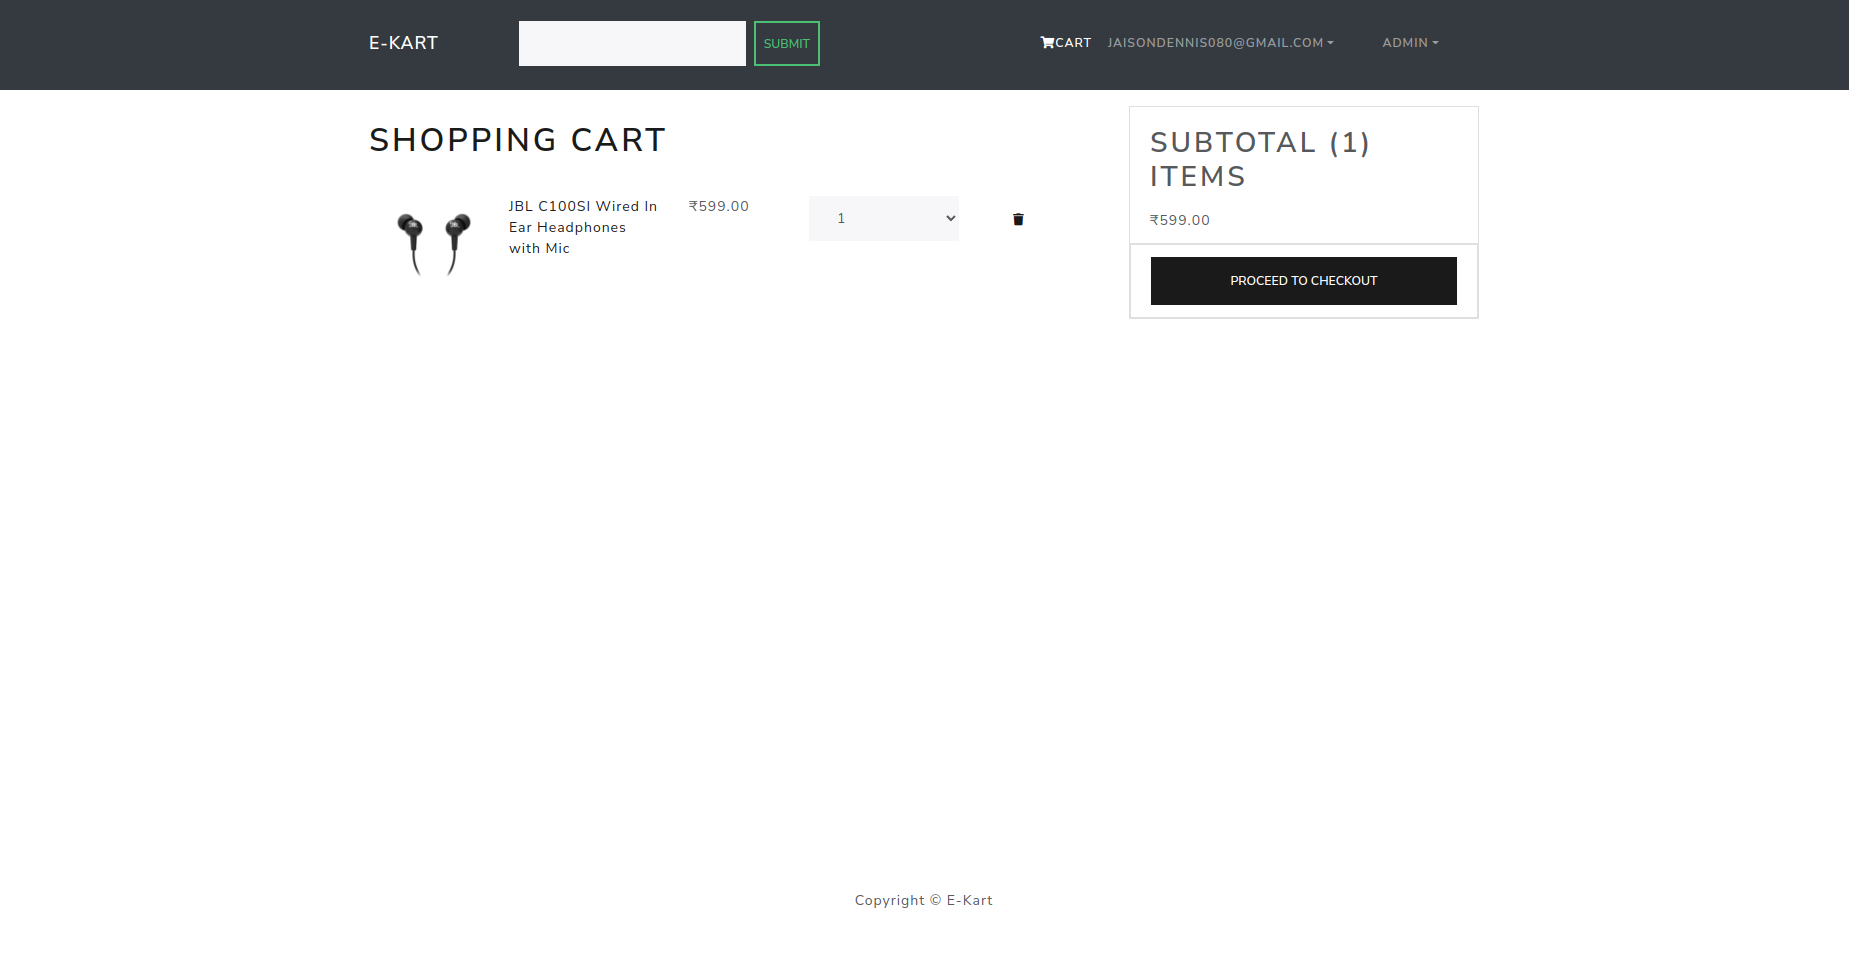
\includegraphics[width=\linewidth]{cart.png}}
	\caption{Shopping Cart}
	\label{fig:s5}
\end{figure}
\begin{figure}[H]
	\fbox{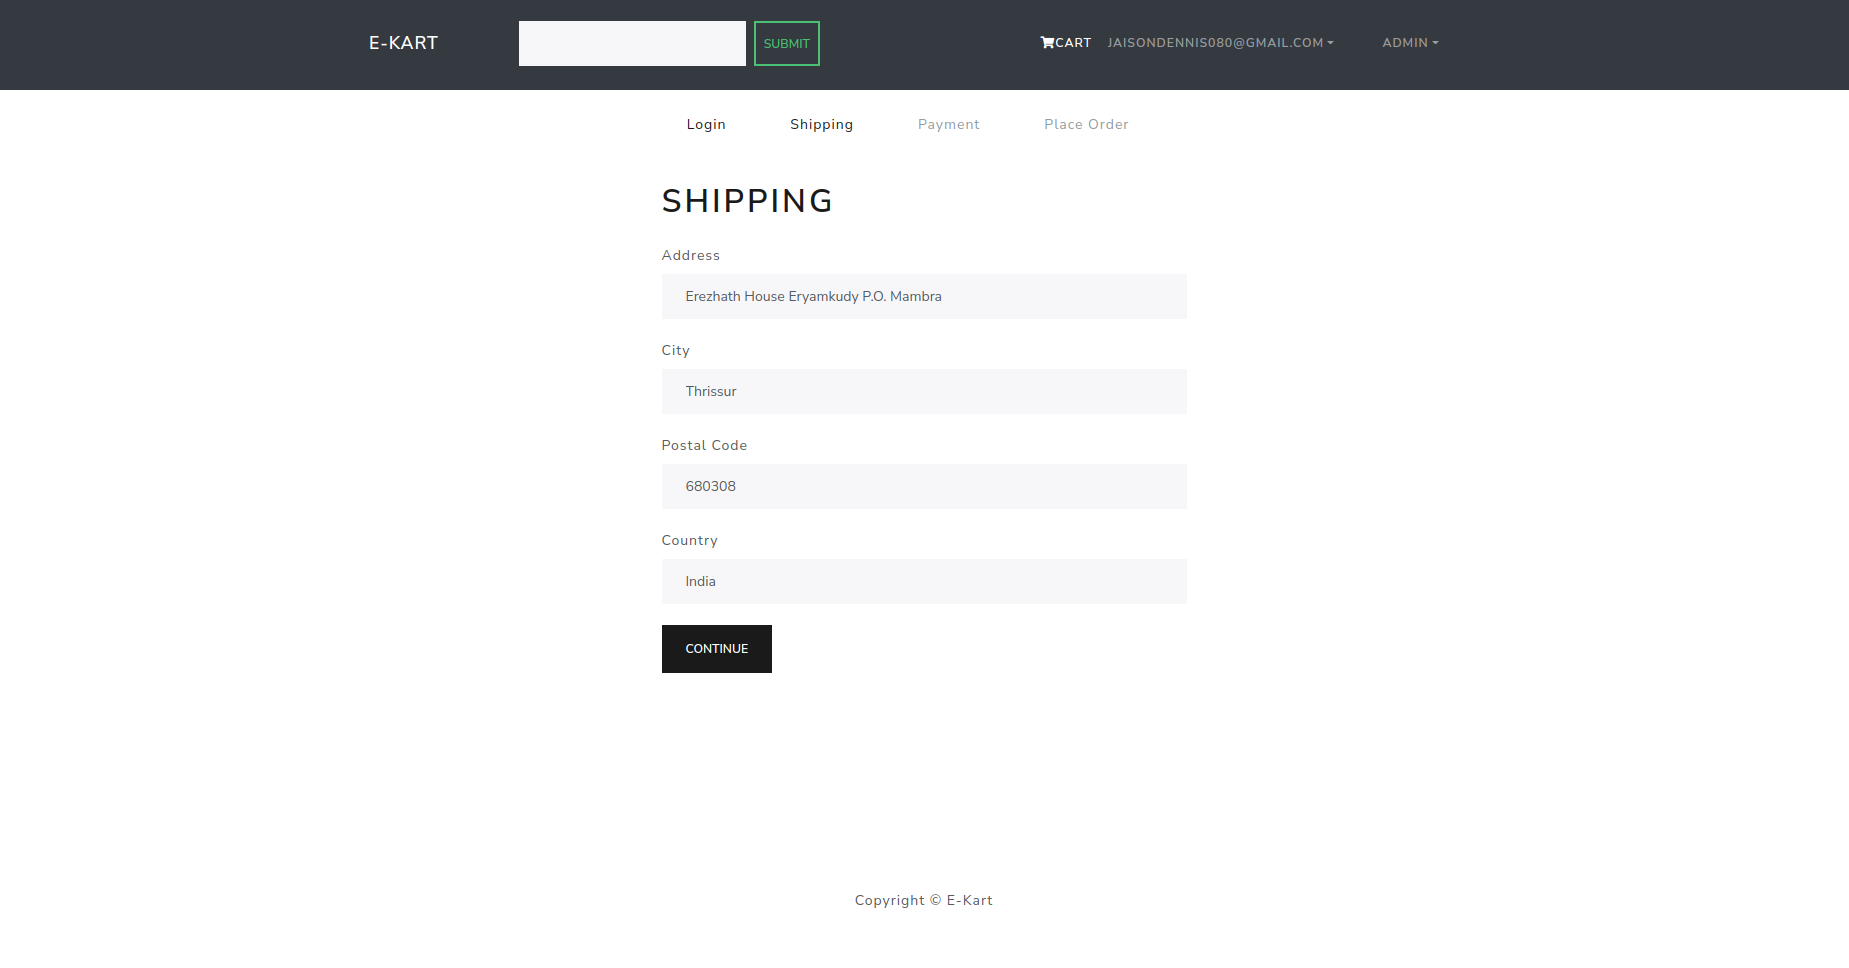
\includegraphics[width=\linewidth]{shipping.png}}
	\caption{Shipping Details}
	\label{fig:s6}
\end{figure} 
\begin{figure}[H]
	\fbox{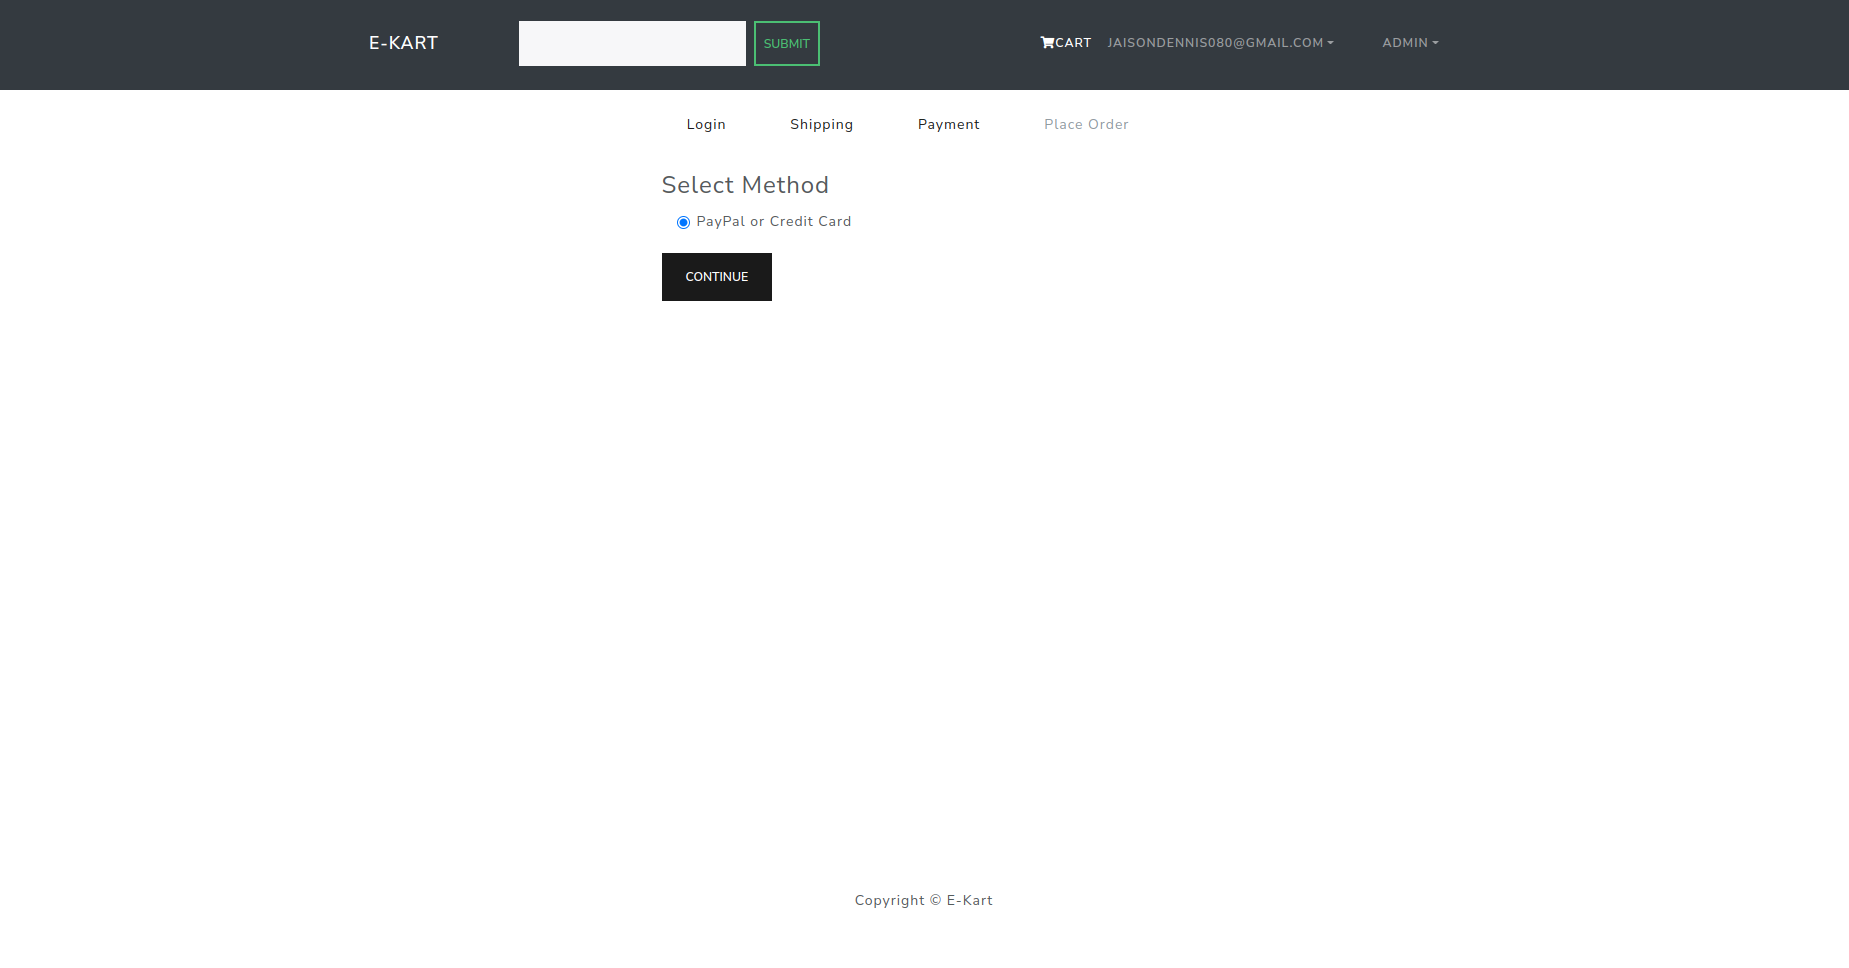
\includegraphics[width=\linewidth]{payment.png}}
	\caption{Payment Method}
	\label{fig:s7}
\end{figure}
\begin{figure}[H]
	\fbox{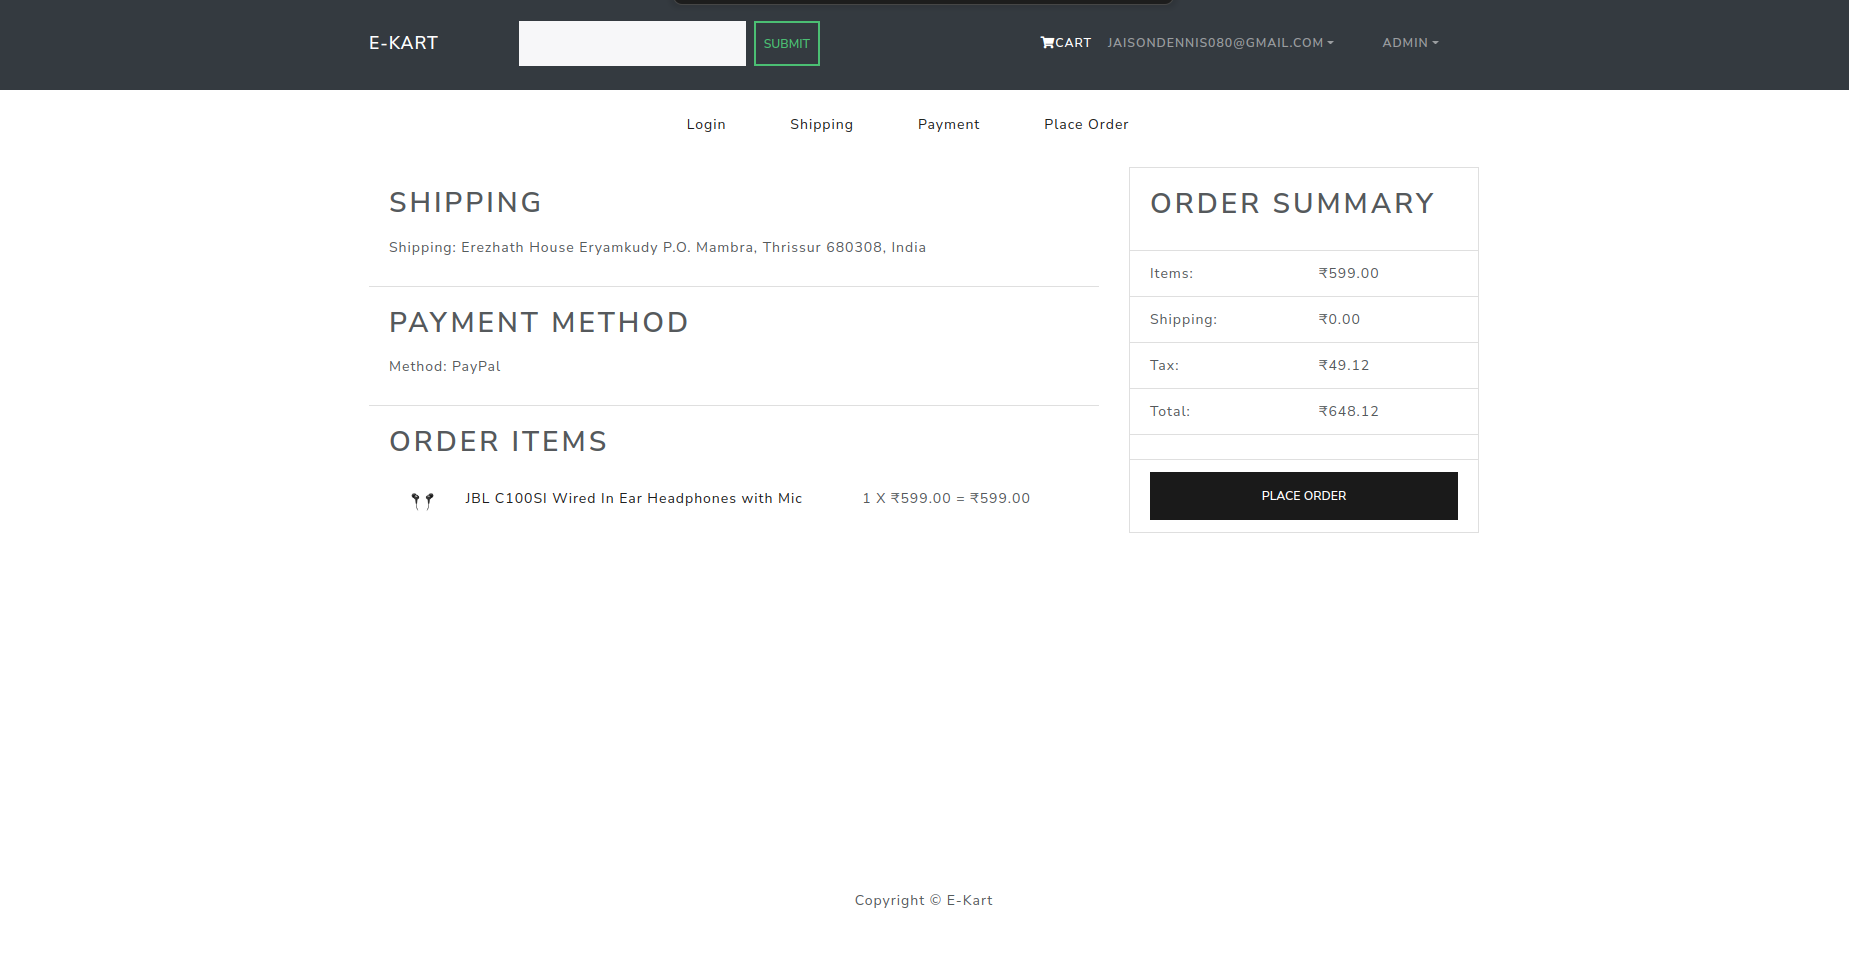
\includegraphics[width=\linewidth]{confirm.png}}
	\caption{Confirm Order}
	\label{fig:s8}
\end{figure}
\begin{figure}[H]
	\fbox{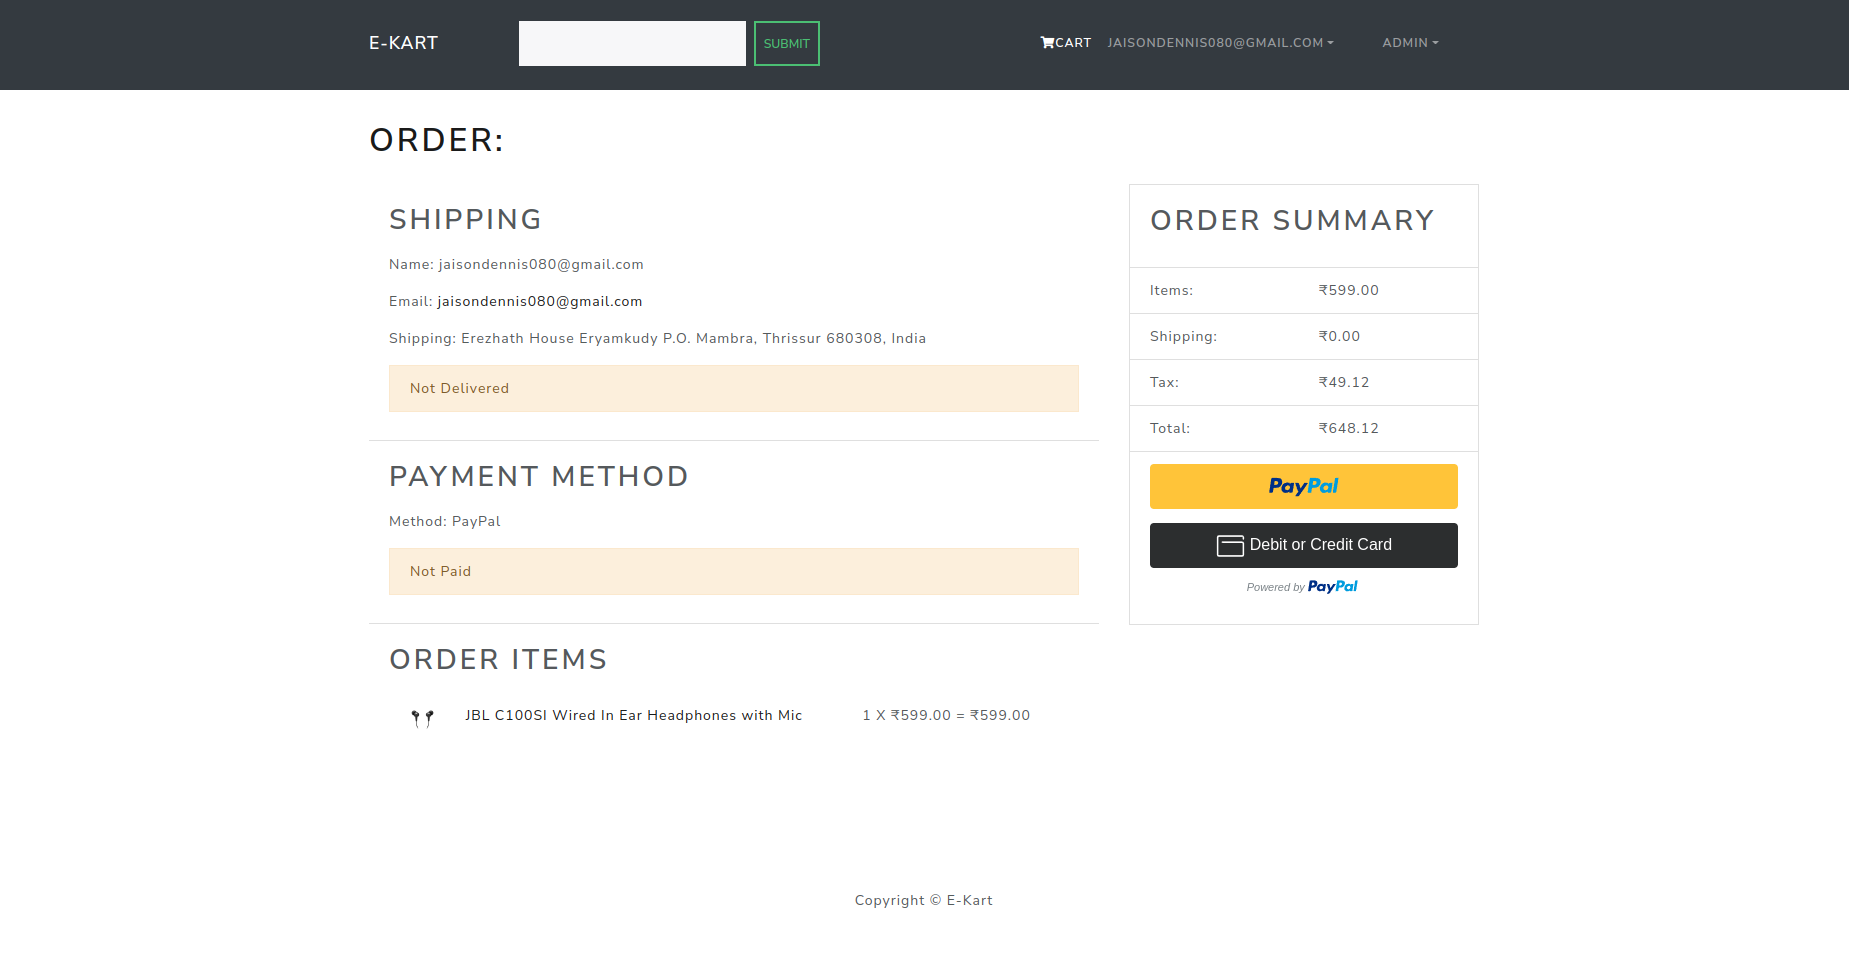
\includegraphics[width=\linewidth]{status.png}}
	\caption{Order Status}
	\label{fig:s9}
\end{figure}
\begin{figure}[H]
	\fbox{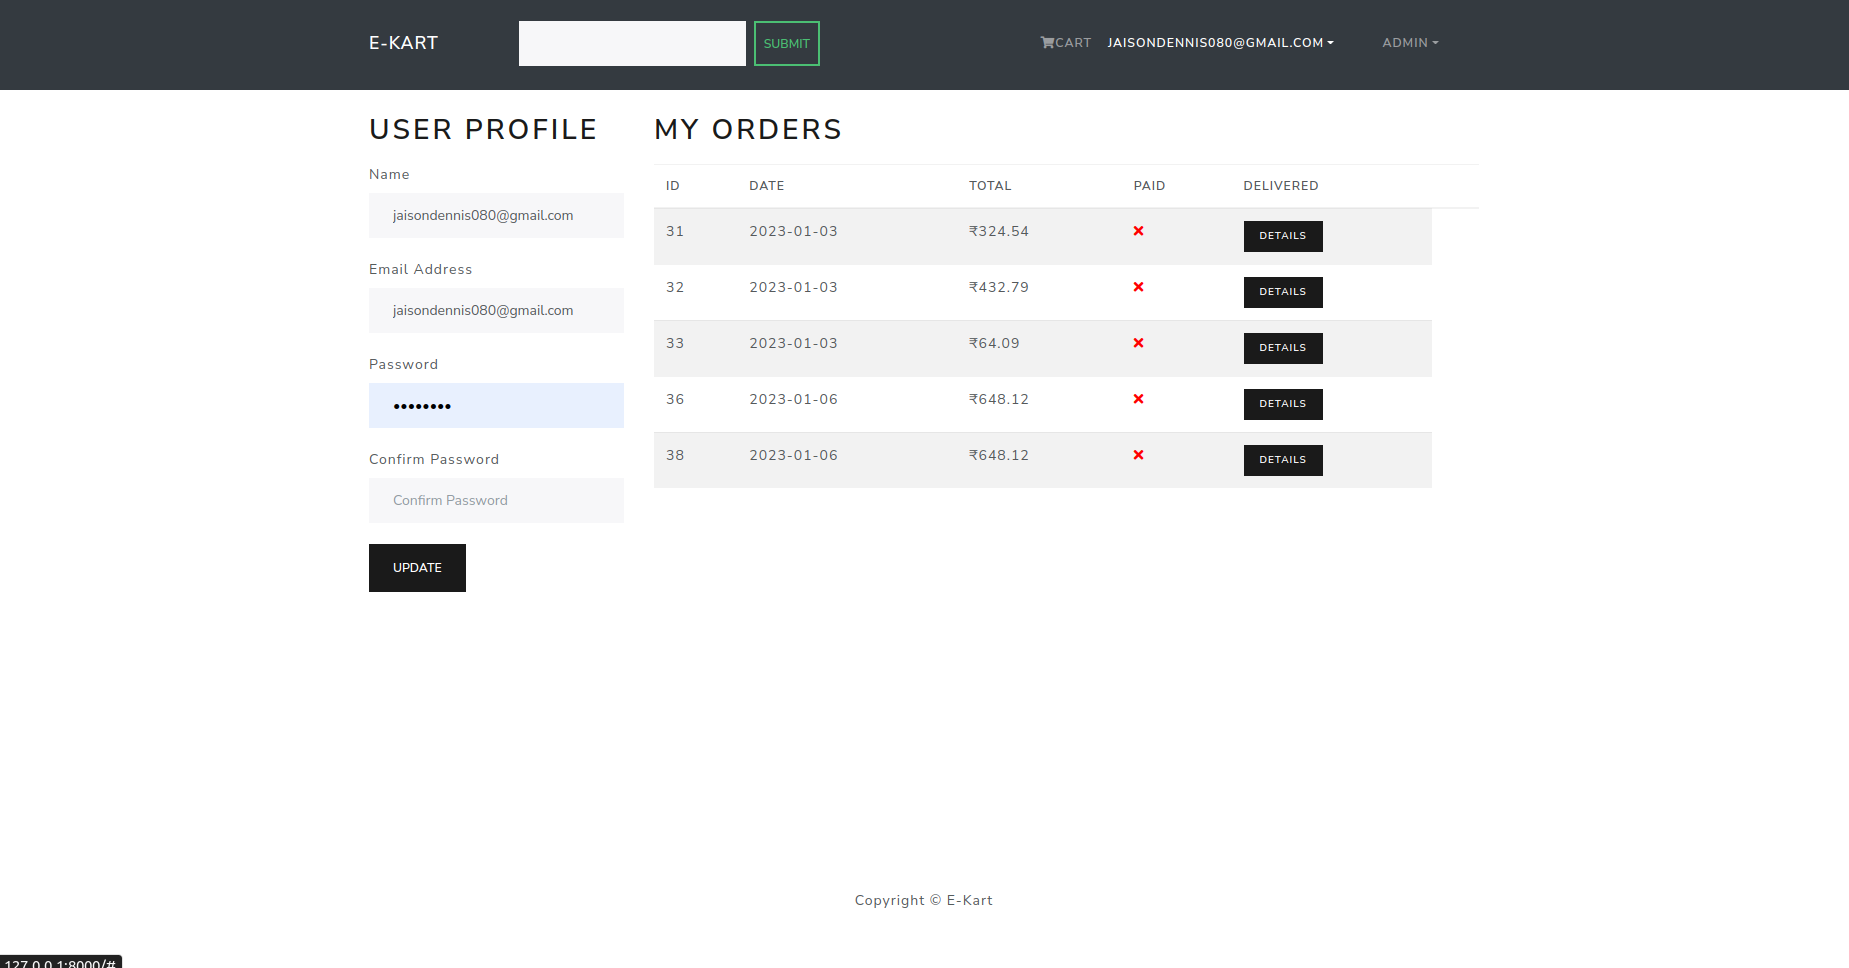
\includegraphics[width=\linewidth]{profile.png}}
	\caption{User Profile}
\end{figure}
\begin{figure}[H]
	\fbox{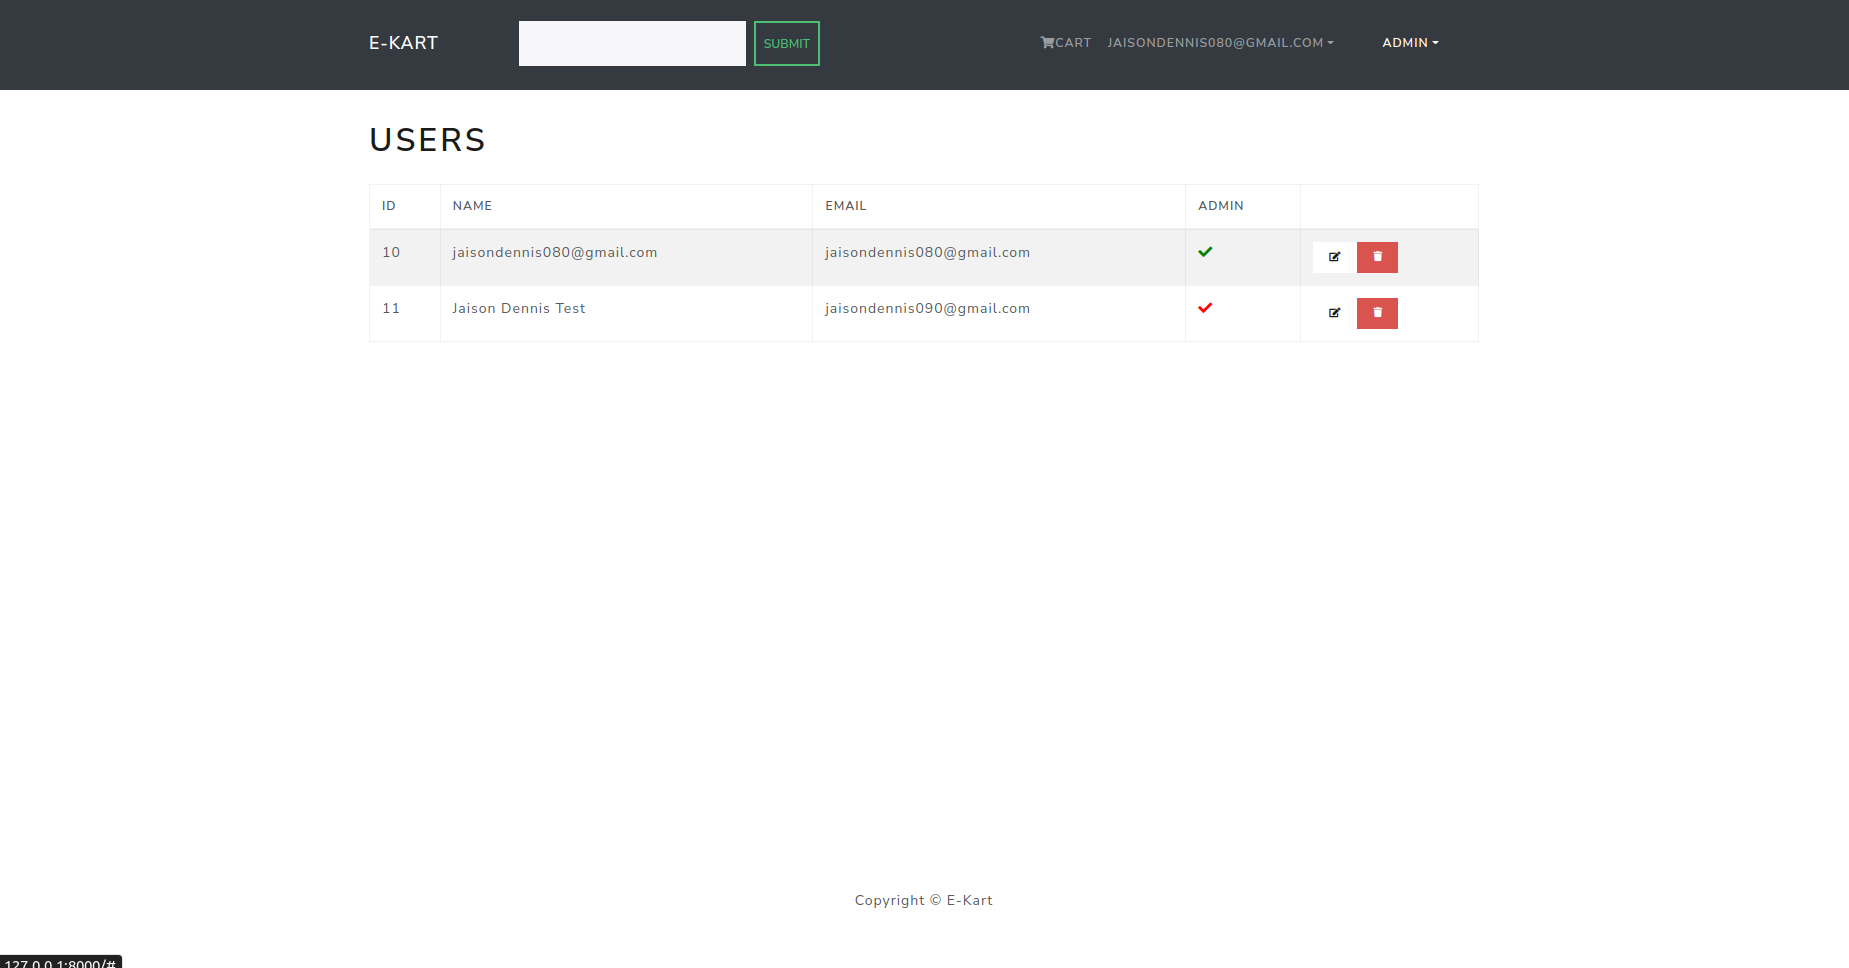
\includegraphics[width=\linewidth]{users.png}}
	\caption{View Users}
\end{figure}
\begin{figure}[H]
	\fbox{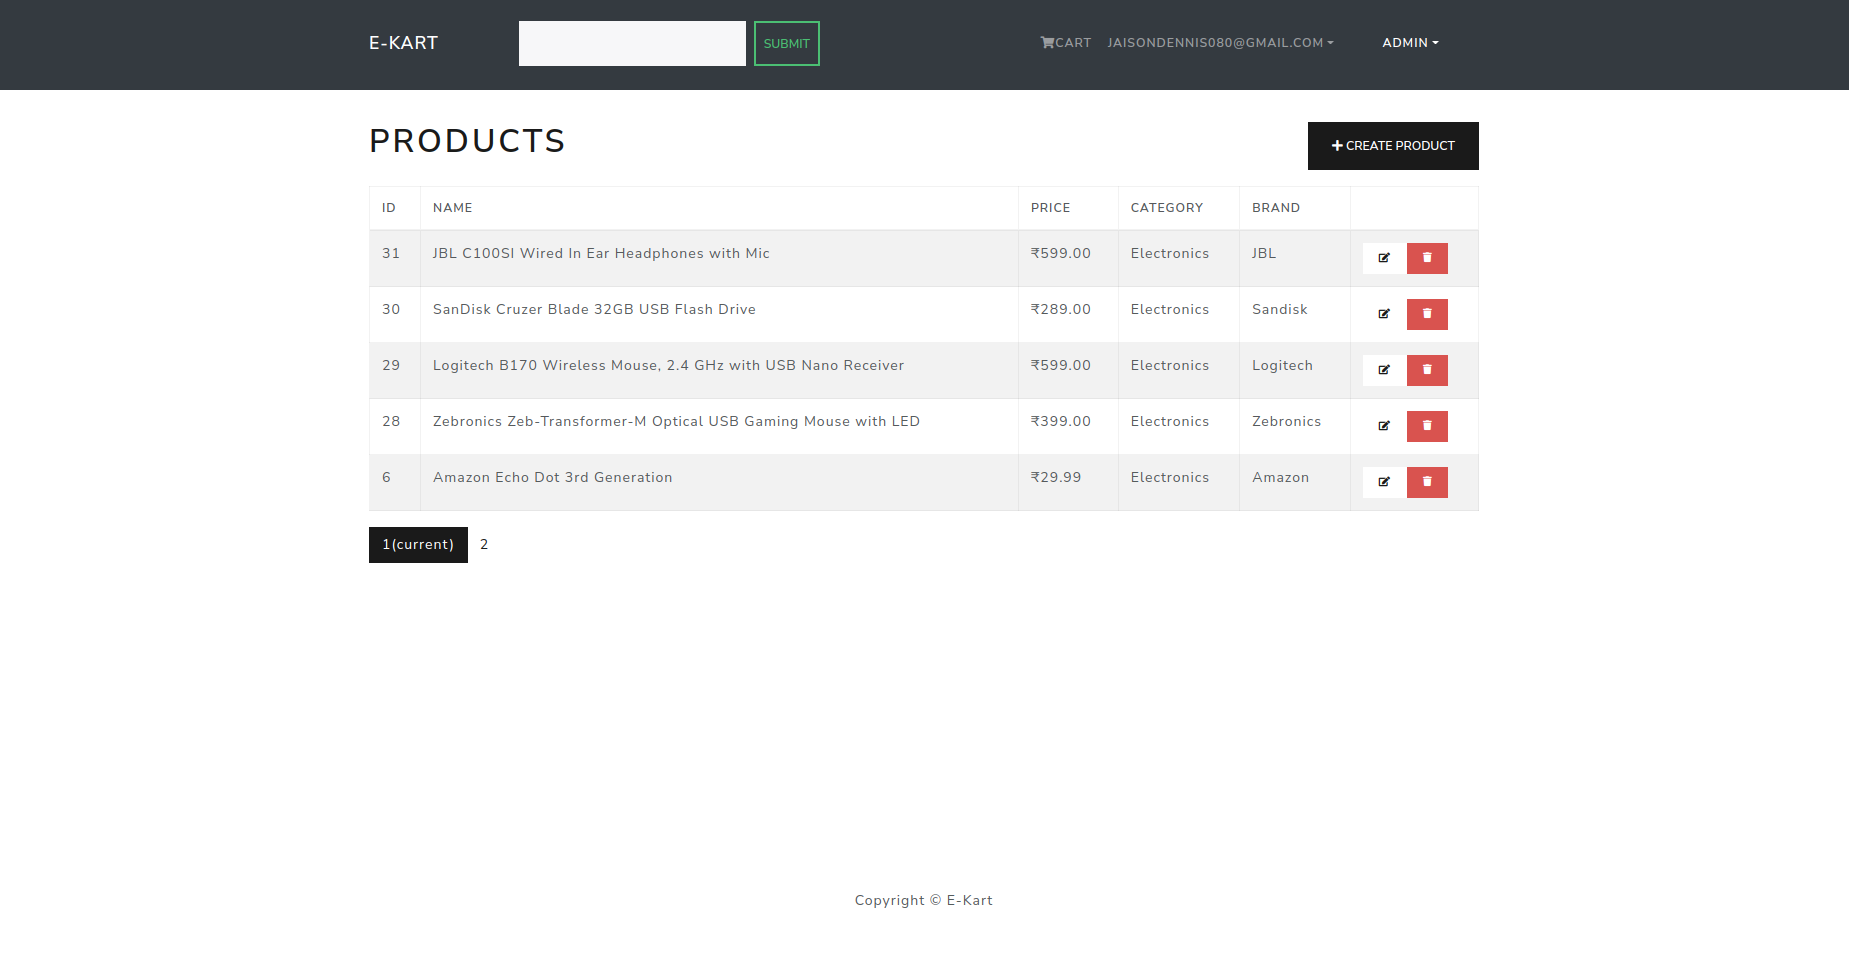
\includegraphics[width=\linewidth]{products.png}}
	\caption{View Products}
\end{figure}
\begin{figure}[H]
	\fbox{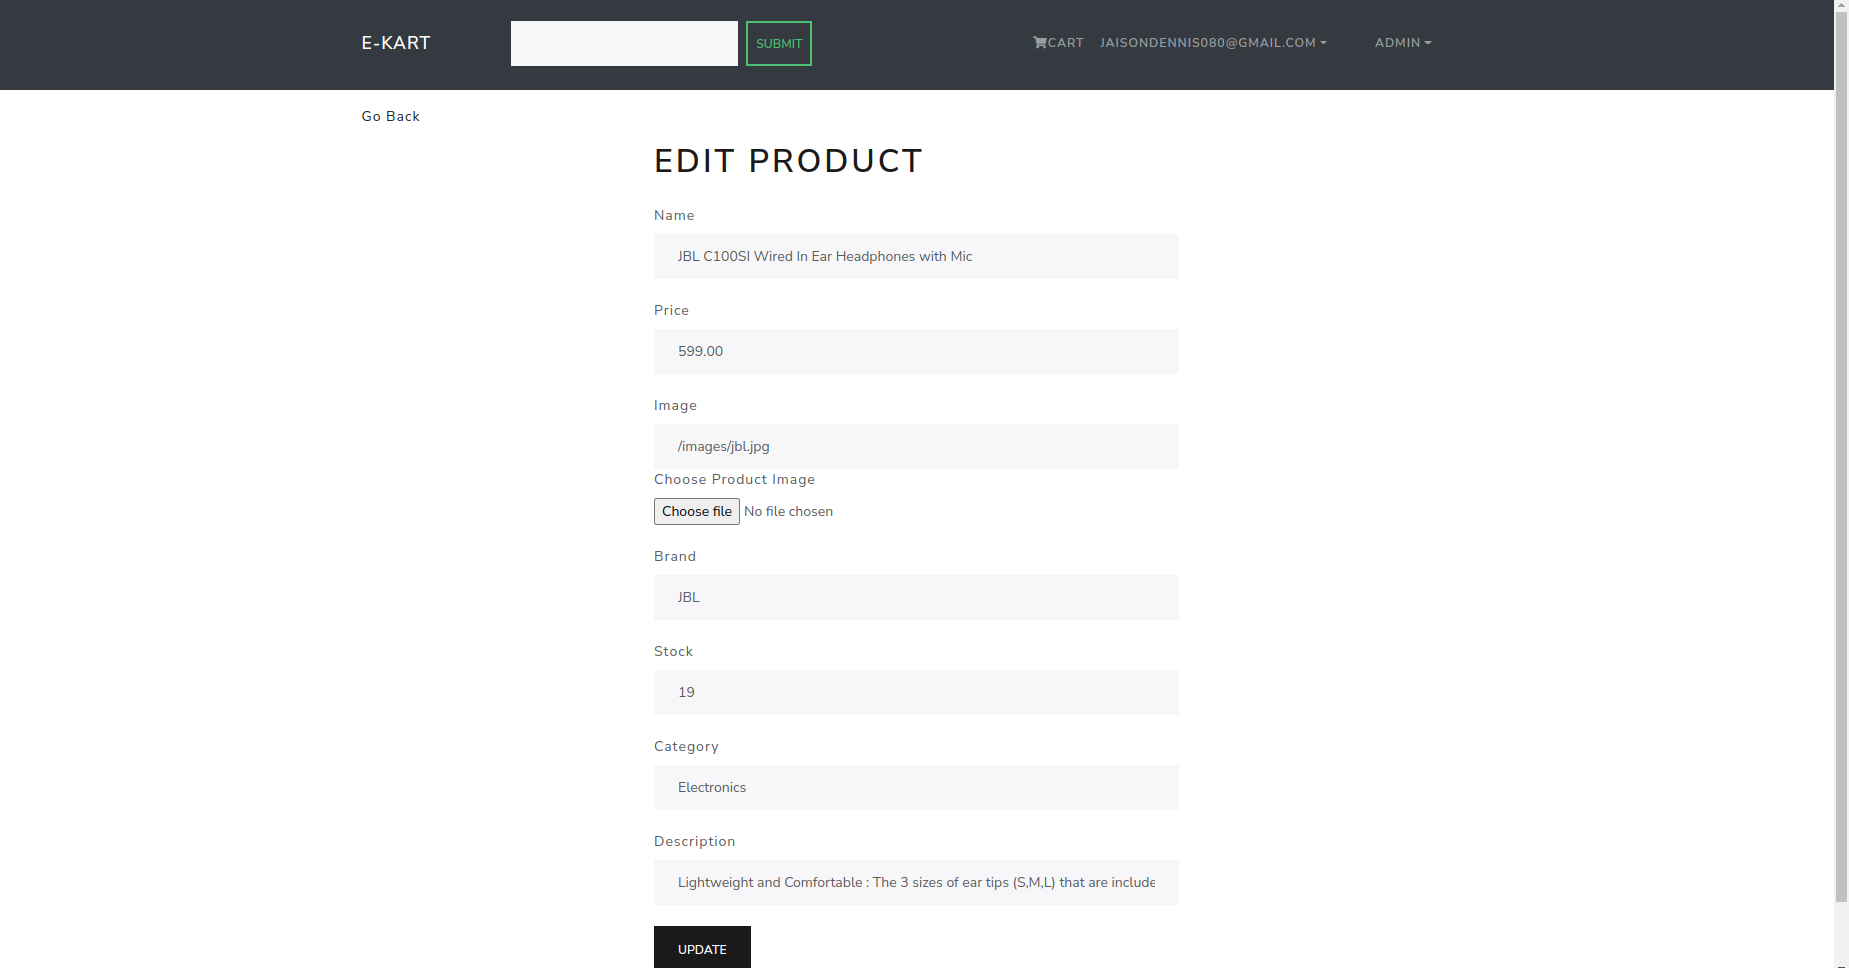
\includegraphics[width=\linewidth]{editproduct.png}}
	\caption{Edit Product}
\end{figure}
\begin{figure}[H]
	\fbox{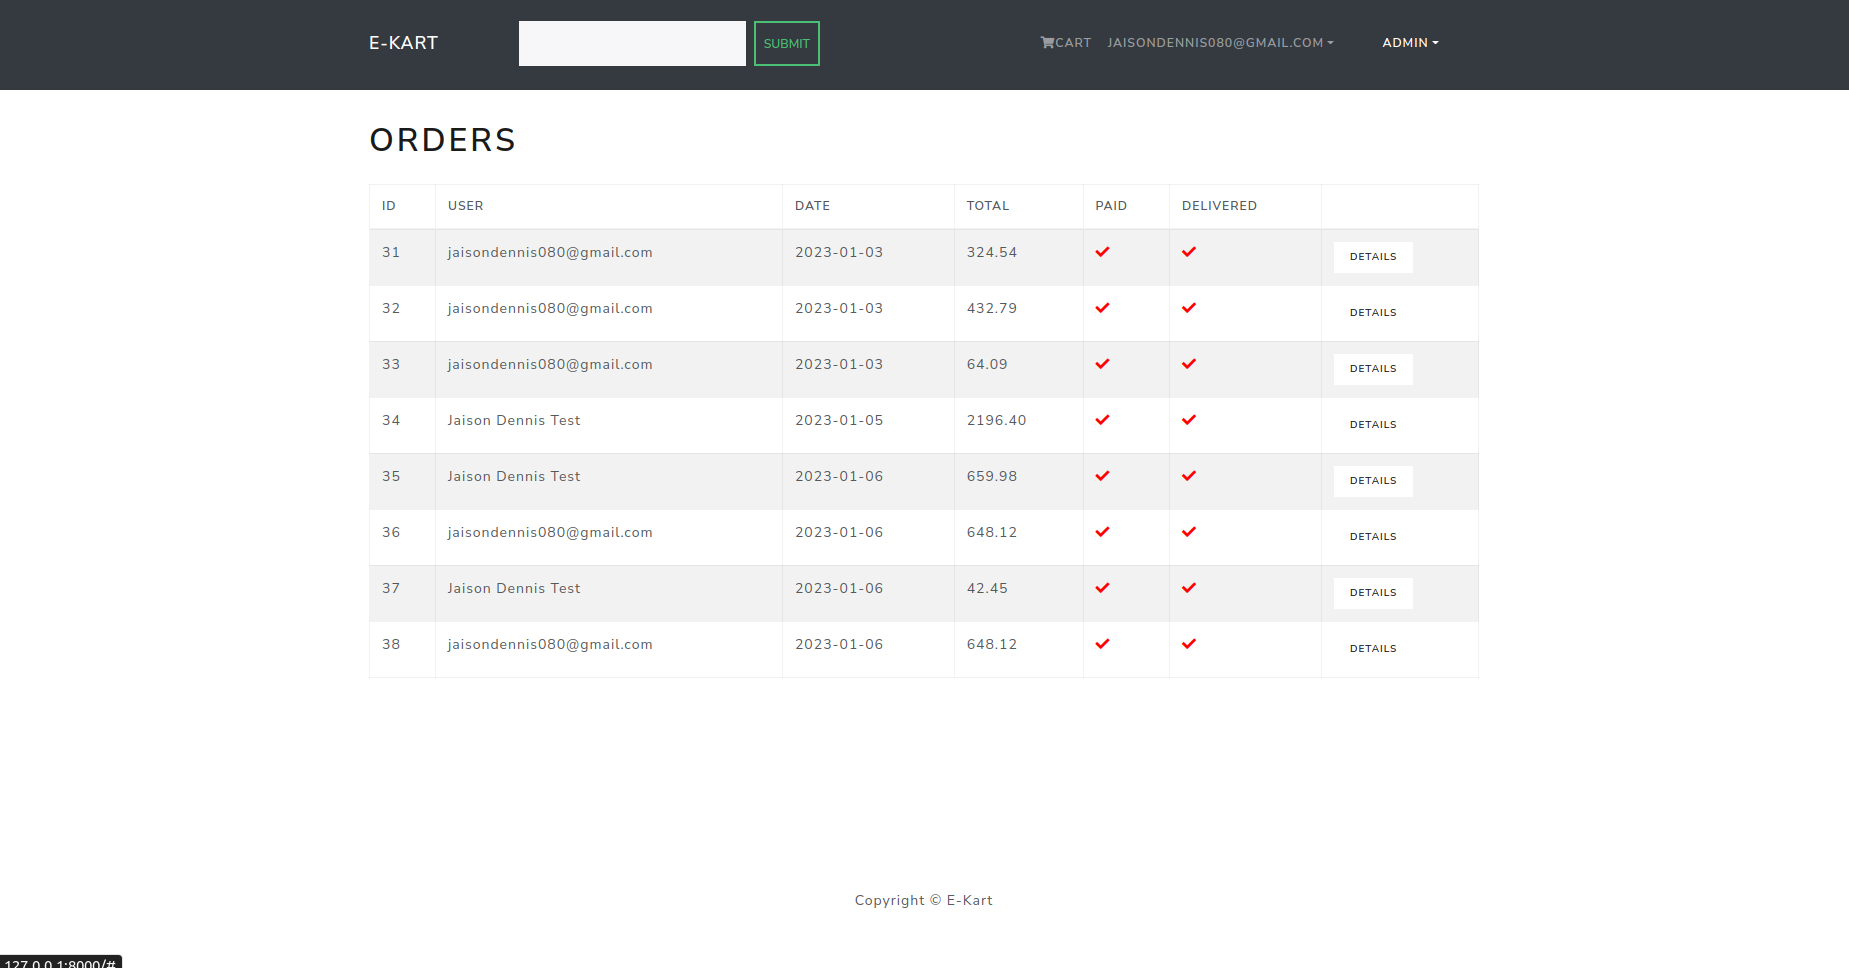
\includegraphics[width=\linewidth]{orders.png}}
	\caption{View Orders}
\end{figure}
 \chapter{Conclusion}
 \label {con}


 

   
%\begin{thebibliography}{999}
%\addcontentsline{toc}{chapter}{References}
%\bibitem{sas}  M Sasikumar, Dinesh Shikkare, P Ravi Prakash: 
%	Introduction to Parallel Processing: First Edition, PHI, New Delhi, 2000
%\bibitem{raj} V Rajaraman. S SivaRama Murthy: 
%	Parallel Computer Architecture and Programming: PHI, New Delhi, 2000
%\bibitem{dav} David HM Spector: Building Linux Clusters: O'Reilly \& associates, 
%CA, USA, 2000
%\bibitem{bar} Thomas C Bartee: Introduction to Computer Science: Third Edition, 
%McGraw-Hill, New York, 1975
%\bibitem{nlb} http://www.netlib.org/pvm3/: PVM software source
%
%\end{thebibliography}
\begin{thebibliography}{999}
\addcontentsline{toc}{chapter}{References}

\bibitem{re1} Shih-Chia Huang, Fan-Chieh Cheng, and Yi-Sheng Chiu, "\textit{Efficient Contrast Enhancement Using Adaptive Gamma Correction With Weighting Distribution}", IEEE TRANSACTIONS ON IMAGE PROCESSING, VOL. 22, NO. 3,pp.1032-1041, MARCH 2013
\bibitem{re2} Rafael C. Gonzalez and Richard E. Woods. \textit{Digital Image Processing}. Pearson Education, Third edition, 2009
\bibitem{re3} William K. Pratt, \textit{Digital Image Processing: PIKS Inside},  Wiley-Interscience Publication, Third Edition.  2001 

\end{thebibliography}


\end{document}
